\newpage
\subsection{Drehmoment bei variabler Drehzahl}\label{subsec:DrehmomentDrehzahl}
Um zu beweisen, dass der Motor die erforderliche Leistung erbringt, wird das Drehmoment in Abhängigkeit der Drehzahl untersucht.
Die Bedingungen, mit welchen der Versuch durchgeführt wurde, können der Tabelle \ref{tab:Drehmoment/Drehzahl} entnommen werden.

\begin{table}[H]
\centering
\begin{tabular}{C{4cm} C{4cm} C{3cm}} 
\multicolumn{3}{c}{\textbf{Versuchsbedingungen}} \\
{Messgrösse}& {Bedingung} & {Wert}\\ \hline\hline 
Spannung (DC)   & nachgeregelt &   96 V     \\
Strom (DC)   & gemessen &   37.8-128 A     \\
Leistung (AC)   & gemessen &   1702-8870 W    \\
Drehzahl   & variiert &   614-2954 RPM    \\
Drehmoment-Sollwert   & nachgeregelt &   32 Nm    \\
Motor-Temperatur   & vernachlässigt &   -    \\
Controller-Temperatur   & vernachlässigt &   -    \\
\end{tabular}
\caption{Versuchsbedingungen Drehmoment/Drehzahl-Versuch}\label{tab:Drehmoment/Drehzahl}
\end{table}

Das Drehmoment an der Welle des BLDC-Motors wird mit der Formel \ref{eq:LeistungDrehmoment} in Abhängigkiet zur Leistung und der Drehzahl des Motors ermittelt. Die daraus ermittelte Kurve ist in der Abbildung \ref{fig:drehmoment/drehzahl} (blaue Kurve) ersichtlich. Da die asynchrone Maschine ebenfalls nicht ideal arbeitet und deswegen Verluste aufweist, wird bei dieser ein Wirkungsgrad von 90\% angenommen (rote Kurve).

\begin{equation}
\centering
P = M \cdot \omega = M \cdot 2 \cdot \pi\cdot f
\label{eq:LeistungDrehmoment}
\end{equation}
$P$\quad Leistung		\\
$M$\quad Drehmoment  \\
$\omega$\quad Winkelgeschwindigkeit\\
$f$\quad Frequenz	\\

\begin{figure}[H]
	\centering
	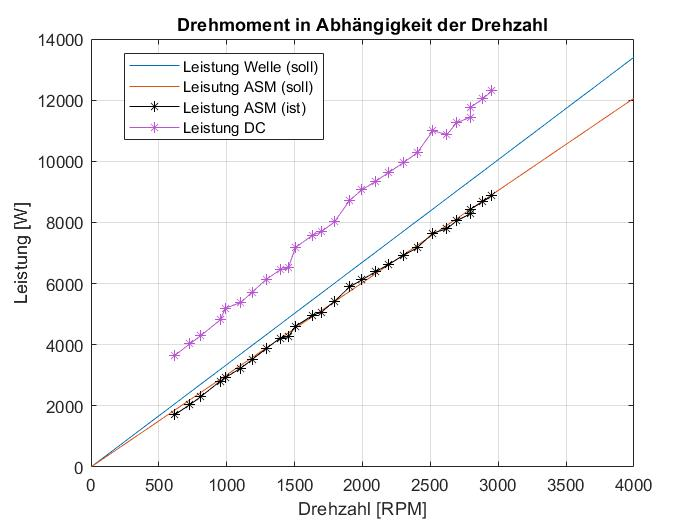
\includegraphics[width=0.9\linewidth]{drehmoment_drehzahl.jpg}
	\caption{Drehmoment in Abhängigkeit der Drehzahl}\label{fig:drehmoment/drehzahl}
\end{figure}

Bei diesem Versuch ist ersichtlich, dass es möglich ist, die erforderliche Leistung (schwarze Punkte) im Drehzahlbereich zwischen 600 und 3000 RPM (engl. revolutions per minute; \glqq Umdrehungen pro Minute\grqq) zu erreichen. Die aufgenommene Leistung auf der DC-Seite (violette Punkte) ist dabei proportional zur abgegebenen Leistung angestiegen und erreicht bei 3000 RPM einen Wert von über 12kW.

\newpage

In der Abbildung \ref{fig:drehmoment/StromSpannung} sind die Spannung, der Strom und die Sollwertvorgabe für die Ansteuerung während des Versuchs ersichtlich. Die Spannung ist auf $96V_{DC}$ nachgeregelt (blaue Punkte) worden, damit diese für den Versuch konstant bleibt. Der Strom (rote Punkte) und der Sollwert für die Ansteuerung (schwarze Punkte) wurden ebenfalls während des Versuchs dokumentiert.


\begin{figure}[H]
	\centering
	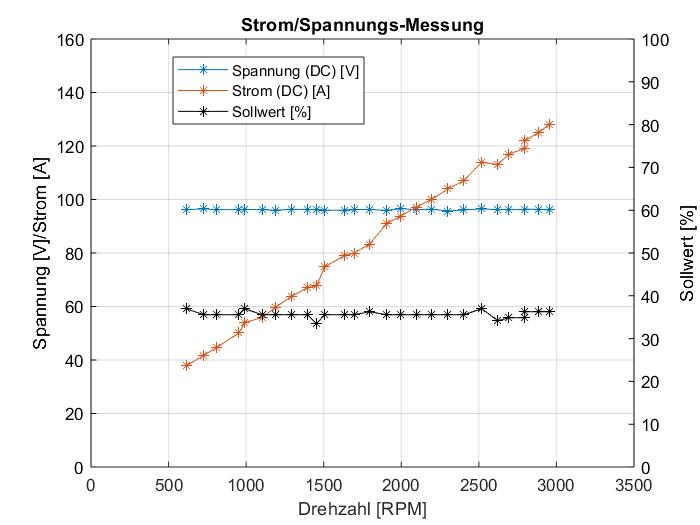
\includegraphics[width=0.9\linewidth]{drehmoment_StromSpannung.jpg}
	\caption{Spannung und Strom während des Drehmomentversuchs}\label{fig:drehmoment/StromSpannung}
\end{figure}

Der Strom kann mit guter Näherung als linear zur Drehzahl bei gleichbleibendem Drehmoment betrachtet werden. Dadurch ergibt sich bei 3800 RPM ein Strom von ca. 160A, was mit den Werten aus dem Datenblatt des Motors korreliert \cite{MotorData}. Diese maximale Leistung konnte mit diesem Versuchsaufbau jedoch nicht getestet werde, da dieser nur für 11kW ausgelegt ist (Kapitel \ref{subsec:Versuchsaufbau}).

Bei diesem Versuch ist ebenfalls ersichtlich, dass die Sollwertvorgabe über den Drehzahlbereich nur kleine Abweichungen aufweist und daher in guter Näherung als konstant betrachtet werden kann. Die Sollwertvorgabe wurde in Prozent des Minimums (1,2V) und des Maximums (4V) angegeben. Eine genauere Analyse des Sollwertvorgabe ist im Unterkapitel \ref{subsec:Steuerkennlinie} bei der Validierung der Steuerkennlinie ersichtlich.
